%% présentation générale
%% architecture





\begin{frame}{Introduction}

  \begin{block}{Rewriting system}

    A method to modelize, in general, the operations of replacing
    subterms in a term by others.\\
    ~\\

    \emph{ie. reduction step of a language semantic, propositionnal
      logic De Morgan's laws, Peano's arithmetic}
    
  \end{block}

  
\end{frame}

\begin{frame}{Rewriting system}

  \begin{block}{Definition}
    
    \begin{itemize}
      \item a set of terms 
      \item a set of rules (term * term)
    \end{itemize}

  \end{block}

  Rewrite a term : applying rules according to a predefined
  \textcolor{red}{strategy} on a given term by \textcolor{blue}{matching} and \textcolor{blue}{replacing} its subterms.

  ~\\
  For instance : \\
  Rule : \texttt{Sub(Add(X))} $\rightarrow$ \texttt{X}\\
  ~\\
  \textcolor{blue}{\texttt{Sub(Add(0))}} $ \rightarrow $ \textcolor{blue}{\texttt{0}}

\end{frame}


\begin{frame}{Non-Linear Nominal Rewriting}
  
  \begin{block}{Nominal}
    There is a distinction between atoms (variables of the language)
    and placeholders/meta-variables (the suterm to replace).
  \end{block}

  \begin{block}{Non-Linear}
    Two instances of the same placeholder
    can appear in the left-hand side of the rule. 
  \end{block}
  
\end{frame}



\begin{frame}{\textcolor{red}{No}minal \textcolor{red}{Work}bench}

  The only rewriting workbench implementing : \\
  \textcolor{blue}{non-linear pattern matching} + \textcolor{blue}{nominal rewriting}

  \begin{block}{Features}
  \begin{itemize}
    \item \textcolor{red}{A simple language} for rewriting systems
    \item Write complexe \textcolor{red}{strategies} with an
      expressful language
    \item Run rewriting operations on terms in an \textcolor{red}{interactive top-loop}
  \end{itemize}
  \end{block}
  
\end{frame}


\begin{frame}{Architecture}

\begin{figure}[h]
\begin{center}
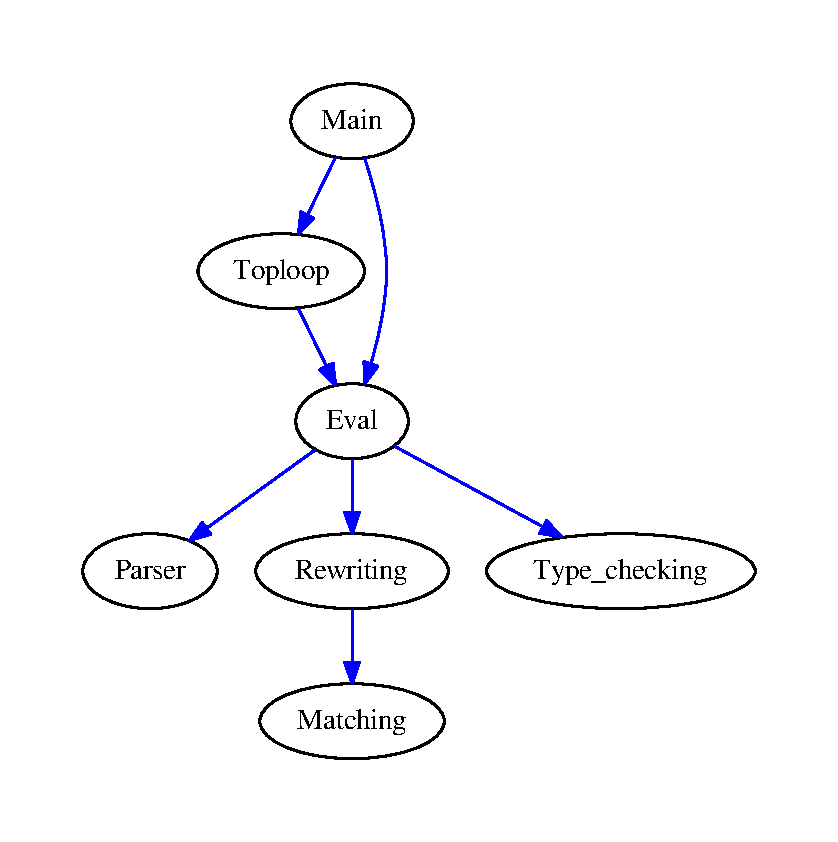
\includegraphics[ height=0.9\textheight]{imports/architecture.pdf}
\end{center}
\end{figure}

\end{frame}


\begin{frame}{Abstract Syntax Trees Architecture}

\begin{figure}[h]
\begin{center}
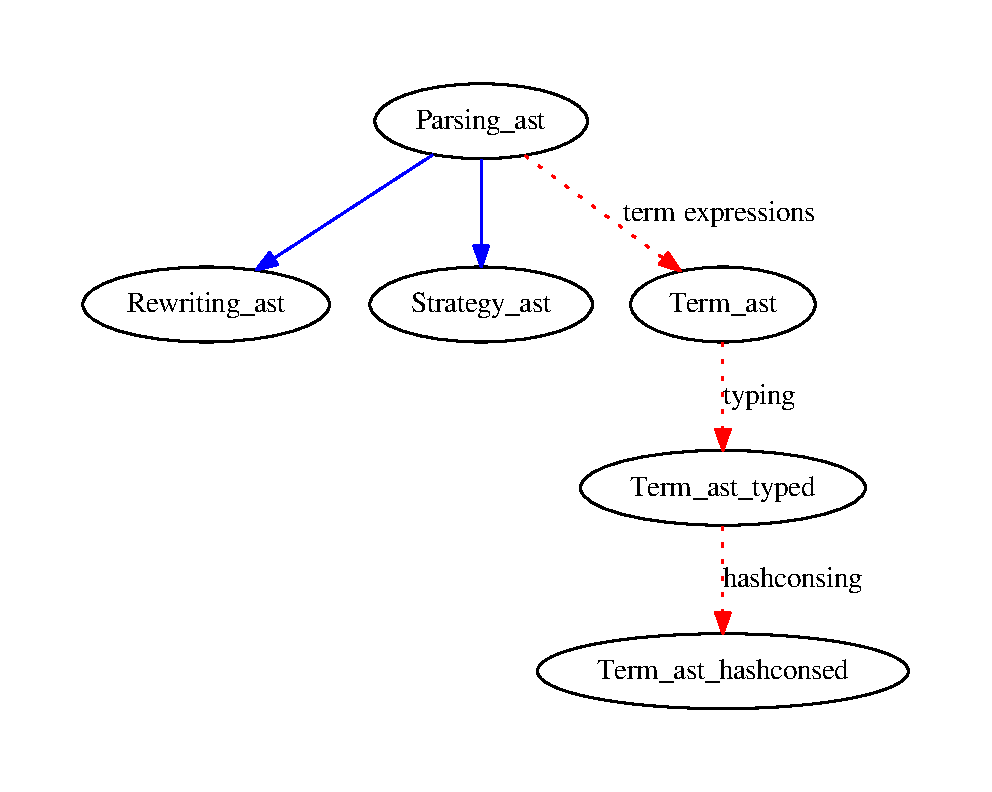
\includegraphics[ height=0.7\textheight]{imports/asts.pdf}
\end{center}
\end{figure}

\end{frame}
